\section{Análisis y Desarrollo}

  Se presenta un análisis descriptivo de los datos recolectados sobre el rendimiento académico de los estudiantes de la UTP en relación con el uso de herramientas de inteligencia artificial. Se calculan de acuerdo a los temas vistos en clase.

  % Pregunta 1 - Género
  \input{components/analisis-desarrollo/desarrollo/q1-genero/generoDeLaMuestra.tex}

  % Pregunta 2 - Carrera
  \input{components/analisis-desarrollo/desarrollo/q2-carrera/carrera.tex}
  
  % Pregunta 3 -  Edad
  \newpage
  \input{components/analisis-desarrollo/desarrollo/q3-edad/edadDeLaMuestra.tex}
  
  % Pregunta 14
  \newpage
  \subsection{Empleo en horas a la semana de las I.A.}
\textbf{Tabla de Frecuencias:} \\

\begin{table}[h!]
	\centering
	\renewcommand{\arraystretch}{1.5} 
	\begin{tabular}{l c c c }
		\hline
		{Rango de horas} & {\(f_i\)} & \textit{\(h_i\)}(\%) & \textit{\(x_i\)}\\
		\hline
		Menos de una hora	& 42 & \(55.26\%\) & \(0.5\)	\\
		1 - 5 horas			& 26 & \(34.21\%\) & \(3\)		\\
		6 - 10 horas 		& 6  & \(7.89\%\)  & \(8\)		\\
		11 - 20 horas 		& 2  & \(2.63\%\)  & \(15.5\)	\\
		Más de 20 horas		& 0  & \(0\%\)     & \(23\)		\\
		\hline
		Total				& 76 & \(100\%\) \\
		\hline
	\end{tabular}
	\caption{Empleo de las inteligencias artificiales en horas a la semana}
	\label{tabla:EmpleoEnHoras}
\end{table}

\textbf{Media(\(\bar{x}\)):}
\begin{equation*}
	\bar{x} = \frac{(0.5 \times 42) + (3 \times 26) + (8 \times 6) + (15.5 \times 2) + (23 \times 0)}{76} \approx 2.34
\end{equation*}
La media semanal del uso de las herramientas de inteligencia artificial es de 2.34 horas, este bajo promedio sugiere que, en general, los encuestados no están profundamente ligados al uso de estas herramientas \\ \\

\noindent\textbf{Varianza:} \\
Se usará varianza muestral.
\begin{equation*}
	s^2 = \frac{(0.5 - 2.34)^2 + (3 - 2.34)^2 + (8 - 2.34)^2 + (15.5 - 2.34)^2 + (23 - 2.34)^2}{75} \approx 8.48
\end{equation*} \\

\begin{minipage}[t]{0.5\textwidth}
	\noindent\textbf{Desviación Estandar:}
	\begin{equation*}
		s = \sqrt{8.48} \approx 2.91
	\end{equation*}
	
\end{minipage}%
\hfill
\begin{minipage}[t]{0.5\textwidth}
	\noindent\textbf{Coeficiente de Variación:}
	\begin{equation*}
		\frac{2.91}{2.34} \times 100 \approx 124.36
	\end{equation*}  
\end{minipage} \\ \\

\noindent\textbf{Interpretación de resultados:}

Las medidas de disperción sugieren que el uso de las herramientas de IA es generalmente bajo entre los encuestados, con una sustancial variabilidad causada por algunos pocos que la usan por extensos periodos de tiempo.
  
  % Pregunta 15
  \newpage
  \subsection{Percepción del Impacto Negativo de la I.A. en el aprendizaje}
\noindent\textbf{Tabla de Frecuencias:}

\begin{table}[h!]
	\centering
	\renewcommand{\arraystretch}{1.5}
	\begin{tabular}{l c c }
		\hline
		Respuestas & \(f_i\) & \(h_i\) \\
		\hline
		Nada & 8 & \(10.53\%\) \\
		Poco & 49 & \(64.47\%\) \\
		De manera significativa & 15 & \(19.74\%\) \\
		Mucho & 4 & \(5.26\%\) \\
		Demasiado & 0 & \(0\%\) \\
		\hline
		Total & 76 & \(100\%\) \\
		\hline
	\end{tabular}
	\caption{Percepción del Impacto Negativo de la I.A. en el aprendizaje}
	\label{tabla:percepciónNegativaEnElAprendizaje}
\end{table}

\noindent\textbf{Moda:} En este caso, es "Poco" puesto que es la respuesta más seleccionada \\ \\
\noindent\textbf{Mediana:} Al tratarse de datos ordinales, la mediana es el punto medio, osea los datos en la posiciones 38 y 39  que tambien pertecen a la respuesta "Poco" \\ \\
\noindent\textbf{Interpretación:} La mayoría de los encuestados considera que el uso de las inteligencias artificiales afecta poco a su aprendizaje
  
  % Pregunta 16
  \newpage
  \subsection{Percepción del porcentaje de tareas automatizadas gracias al uso de herramientas de I.A.}
\noindent\textbf{Tabla de Frecuencias:}
\begin{table}[h!]
	\centering
	\renewcommand{\arraystretch}{1.5}
	\begin{tabular}{l c c c c c}
		\hline
		{Rango de porcentaje} & {\(f_i\)} & \textit{Fi} & \textit{hi}(\%) & \textit{Hi}(\%) & \(x_i\)\\
		\hline
		0\%                  & 3  & 3  & 4.17\%  & 4.17\% & 0\% \\
		1\% - 10\%           & 28 & 31 & 38.89\% & 43.06\% & 5.5\% \\
		11\% - 25\%          & 26 & 57 & 36.11\% & 79.17\% & 18\% \\
		25\% - 50\%          & 10 & 67 & 13.89\% & 93.06\% &37.5\% \\
		Más de un 50\%       & 4  & 71 & 5.56\%  & 100\% & 75\% \\
		\hline
		Total                & 71 &    & 100\%   & & \\
		\hline
	\end{tabular}
	\caption{Distribución de respuestas por porcentaje de tareas automatizadas}
	\label{tabla:porcentaje_IA}
\end{table} \\

\noindent\textbf{Media($\bar{x}$):}
\begin{equation*}
	\frac{(3 \times 0\%) + (5.5 \times 28) + (18 \times 26) + (37.5 \times 10) + (75 \times 4)}{71} \approx 18.268\%
\end{equation*}

\noindent\textbf{Varianza:}
\begin{equation*}
	\frac{(0-18.268)^2 + (5.5-18.268)^2 + (18-18.268)^2 + (37.5 - 18.268)^2 + (75 - 18.268)^2}{70} \approx 58.36
\end{equation*}

\begin{multicols}{2}
	\noindent\textbf{Mediana(\(M_e\)):}
	\begin{center}
		$11\% + 14(\frac{35.5 - 31}{26}) \approx 13.42\%$
	\end{center}
	\columnbreak
	\vfill
	\noindent\textbf{Desviación Estandar}
	\begin{center}
		$\sqrt{58.36^2} \approx 7.64$
	\end{center}
\end{multicols}

\noindent\textbf{Percentiles:} Se calculan los percentiles para calcular el coeficiente de asimetría de Pearson

\begin{multicols}{2}
	\noindent$P_{75} = 11\% + 14\left(\frac{53.25 - 31}{26}\right) \approx 22.98\%$ \\ \\
	$P_{25} = 1\% + 9\left(\frac{17.75 - 3}{28}\right) \approx 5.74\%$
	\columnbreak
	\vfill
	\noindent$P_{90} = 25\% + 25\left(\frac{63.9 - 57}{10}\right) \approx 42.25\%$ \\ \\
	$P_{10} = 1\% + 9\left(\frac{7.1 - 3}{28}\right) \approx 2.32\%$
\end{multicols}

\begin{multicols}{2}
	\noindent\textbf{Pearson:} La distribución tiene asimetría positiva
	\begin{equation*}
		3\left(\frac{18.268-13.42}{7.64}\right) \approx 1.90
	\end{equation*}
	\vfill
	\columnbreak
	\noindent\textbf{Curtosis:} La distribución es leptocúrtica
	\begin{equation*}
		\frac{22.98-5.74}{42.25-2.32} \approx 0.43
	\end{equation*}
\end{multicols}

\newpage

\noindent\textbf{Gráfico de medidas de forma}
\begin{figure}[h!]
	\centering
	\hspace*{-1.2cm}
	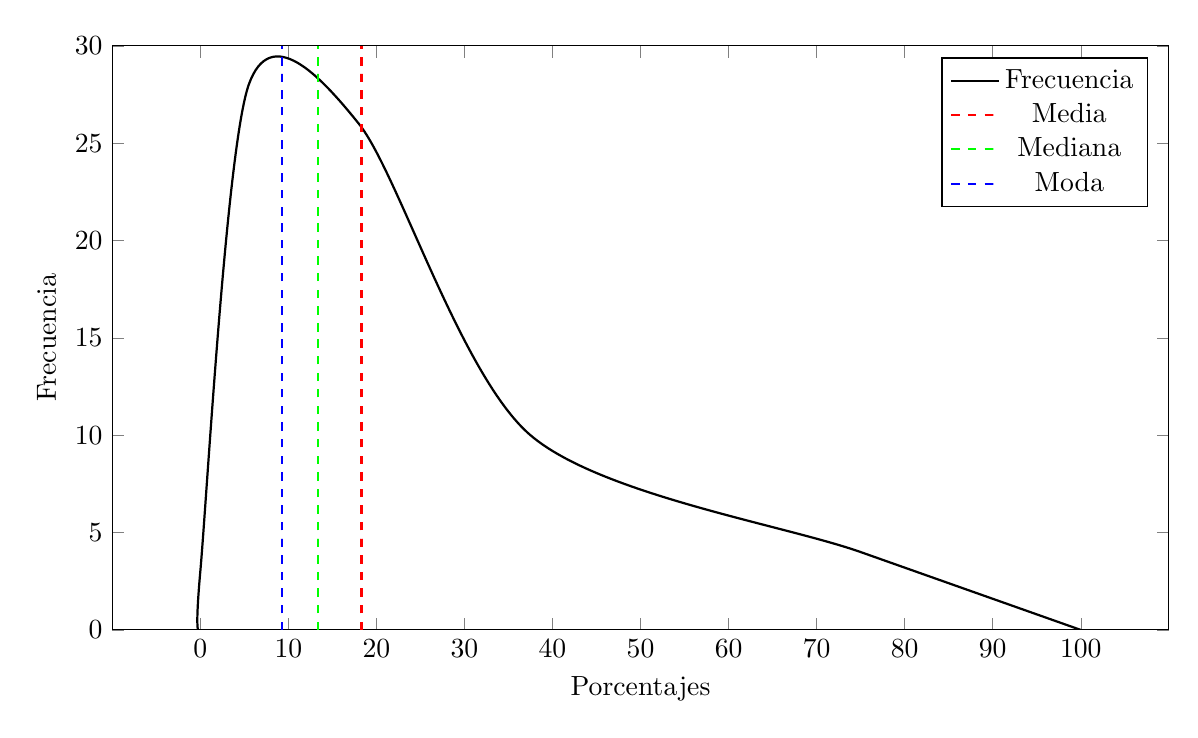
\begin{tikzpicture}
		\begin{axis}[
			width=15cm, height=9cm,
			xlabel={Porcentajes},
			ylabel={Frecuencia},
			xtick={0,10,20,30,40,50,60,70,80,90,100},
			ymin=0, ymax=30,
			grid=none,
			smooth,
			tension=0.5
			]
			\addplot[
			color=black,
			thick
			]coordinates{
				(0,0)
				(0,3)
				(5.5,28)
				(18,26)
				(37.5,10)
				(75,4)
				(100,0)
			};
			
			\addplot[
			color=red,
			thick,
			dashed
			]coordinates{(18.3,0)(18.3,30)};
			
			\addplot[
			color=green,
			thick,
			dashed
			]coordinates{(13.4,0)(13.4,30)};
			
			\addplot[
			color=blue,
			thick,
			dashed
			]coordinates{(9.3,0)(9.3,30)};
			\legend{Frecuencia, Media, Mediana, Moda}
		\end{axis}
	\end{tikzpicture}
	\caption{Distribución Positiva}
\end{figure}

\noindent\textbf{Interpretación de la información:} \\
Los resultados muestran que la mayoría de los participantes percibe un nivel bajo a moderado de automatización de tareas gracias a la IA, con el 38.89\% estimando entre un 1\% y un 10\% de automatización y el 36.11\% entre un 11\% y un 25\%. La media del 18.27\% y la mediana de 13.42\% reflejan esta tendencia, y la ligera asimetría positiva (1.90) indica una mayor concentración de respuestas en los valores bajos, con pocos participantes reportando niveles elevados de automatización. La curtosis leptocúrtica (0.43) sugiere una concentración de respuestas cerca de la media, consolidando la observación de que la mayoría ve un impacto limitado de la IA en sus tareas. En conjunto, estos hallazgos sugieren una implementación de IA aún incipiente en este contexto, con mayor aplicación en tareas específicas y menores porcentajes de automatización.
  
  % Pregunta 16